\subsection{Временные ряды}

    Для демонстрации поведения системы можно использовать временные ряды. Временной ряд позволяет наглядно показать как с течением времени изменяется численность популяции.

    Далее рассмотрим подробнее основные типичные ситуации. Для этого давайте зафиксируем параметр следующим образом: \(\beta = 0.56\). 

    На рисунке \ref{time_series_b_0_56} мы видим, что временные ряды, которые начинаются в \(x_0 = 0.04\) и в \(x_0 = 1.3\) сходятся к нулю. В биологическом смысле это означает, что популяция с течением времени вымирает.

    А теперь зафиксируем начальную численность популяции на уровне \(x_0 = 0.06\). На рисунке \ref{time_series_b_0_56} видно, что при таких начальных условиях популяция увеличивается до некоторого значения. После достижения которого рост численности популяции прекращается. То есть популяция с течением времени стабилизируется.

    Похожую ситуацию мы можем наблюдать на том же рисунке \ref{time_series_b_0_56} при начальном значении \(x_0 = 0.3\). Значения численности популяции тоже сходятся к устойчивому равновесию. Численность снова стабилизируется.
    
    \begin{figure}
        \centering
        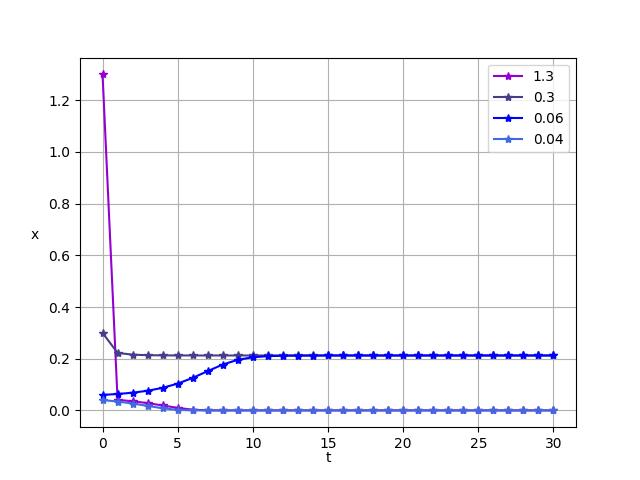
\includegraphics[width=\textwidth]{deterministic/images/time_series_b_0_56.jpg}

        \captionsetup{justification=centering}
        \caption{Временные ряды модели (\ref{origin}) для \(\beta = 0.56\) при различных начальных значениях}
        \label{time_series_b_0_56}
    \end{figure}

    Рассмотрим ситуацию, когда \(\beta = 0.4\) и \(x_0 = 0.1\). На рисунке \ref{time_series_x_0_1_b_0_4} можно заметить, что элементы временного ряда принимают два значения. Это соответствуют циклу порядка 2, который можно увидеть на бифуркационной диаграмме, которую можно увидеть на рисунке \ref{bifurcation}.
    
    \begin{figure}
        \centering
        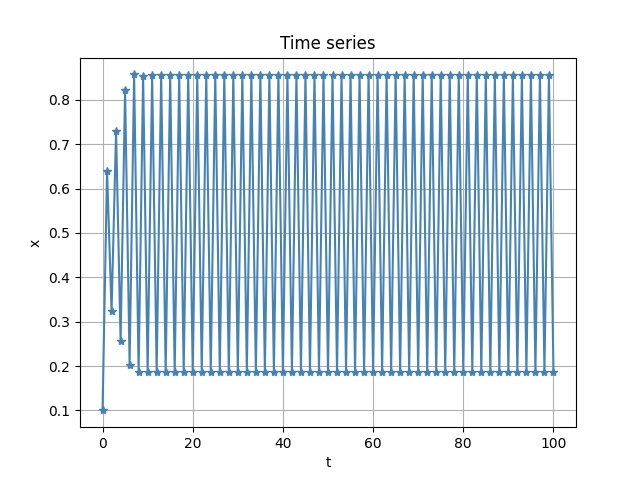
\includegraphics[width=\textwidth]{deterministic/images/time_series_x_0_1_b_0_4.jpeg}

        \captionsetup{justification=centering}
        \caption{Временной ряд модели (\ref{origin}) для \(\beta = 0.4\) и \(x_0 = 0.1\)}
        \label{time_series_x_0_1_b_0_4}
    \end{figure}

    Давайте теперь изменим значение параметра: \(\beta = 0.25\). Начальная численность популяции: \(x_0 = 0.1\). На рисунке \ref{time_series_x_0_1_b_0_25} видно, что нет закономерности, по которой меняется численность популяции. Это поведение соответствуют хаосу.
    
    \begin{figure}
        \centering
        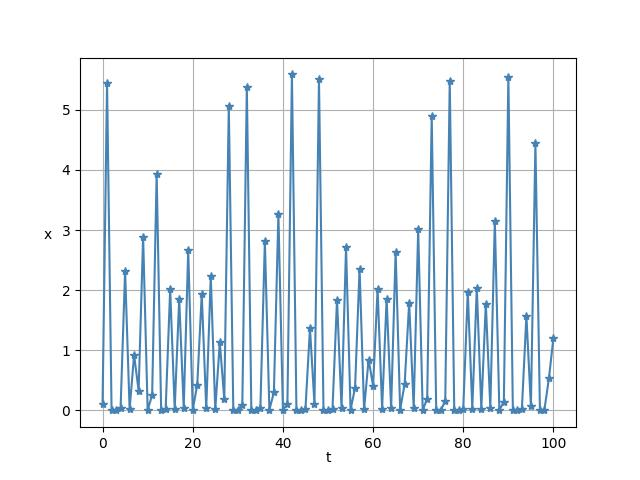
\includegraphics[width=\textwidth]{deterministic/images/time_series_x_0_1_b_0_25.jpg}

        \captionsetup{justification=centering}
        \caption{Временной ряд модели (\ref{origin}) для \(\beta = 0.25\) и \(x_0 = 0.1\)}
        \label{time_series_x_0_1_b_0_25}
    \end{figure}
